\documentclass[10pt]{article}
\usepackage[margin=1.0cm,top=0.75cm,bottom=0.75cm,columnsep=0.5cm]{geometry}
\usepackage[utf8]{inputenc}
\usepackage[T1]{fontenc}
\usepackage{lmodern}
\usepackage{microtype}
\usepackage{multicol}
\usepackage{booktabs}
\usepackage{xcolor}
\usepackage{hyperref}
\usepackage{tikz}
\usetikzlibrary{positioning,arrows.meta,calc}

\definecolor{ucblue}{RGB}{0,51,102}
\definecolor{toolgray}{RGB}{110,110,110}
\hypersetup{colorlinks=true,urlcolor=ucblue,linkcolor=ucblue}
\setlength{\parindent}{0pt}
\setlength{\parskip}{2pt}
\pagestyle{empty}
\newcommand{\head}[1]{\textbf{\color{ucblue}#1}\hspace{0.4em}}
\newcommand{\pendiente}[1]{\textcolor{red}{[PENDIENTE: #1]}}
\newcommand{\VideoURL}{\pendiente{enlace del video}}

\begin{document}

\begin{center}
{\Large\bfseries\color{ucblue} SQL4Business: Deliverable 3 --- sistema de agentes}\\[2pt]
{\small Generative Artificial Intelligence (580694), Universidad de Concepci\'on}\\[1pt]
{\small Aredhel Jim\'enez, Bryan Riquelme, Guido Salazar, Vicente So\~nez}\\[1pt]
{\small C\'odigo: \href{https://github.com/aredhel-jmze/Asistente-SQL-4-Business}{github.com/aredhel-jmze/Asistente-SQL-4-Business}
\quad$\vert$\quad Video: \VideoURL}
\end{center}

\vspace{-4pt}
\begin{center}
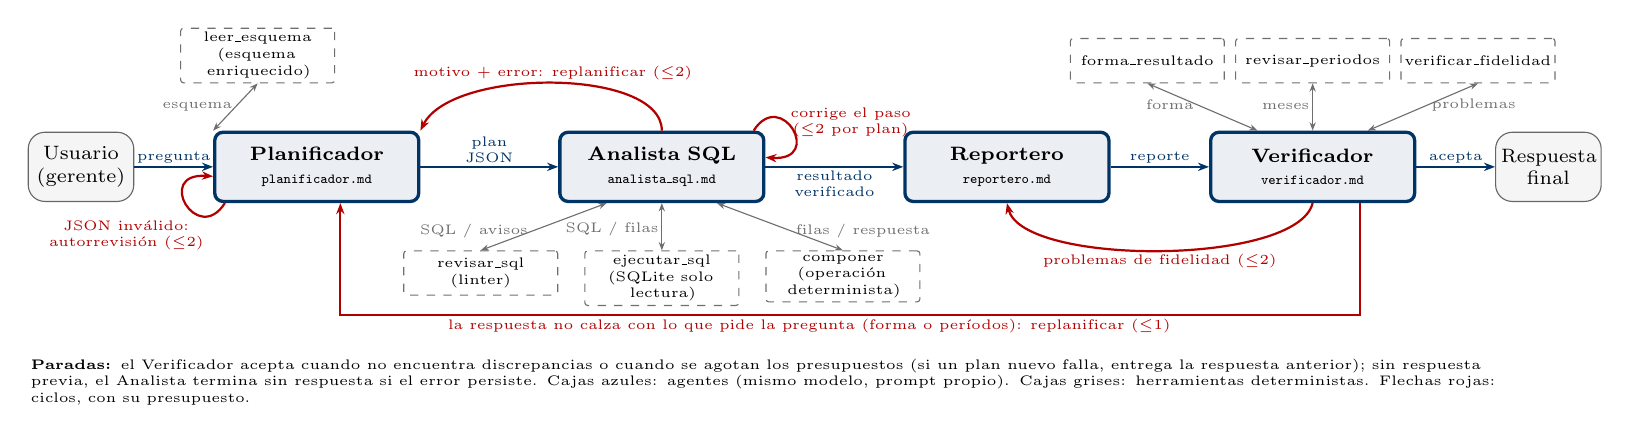
\begin{tikzpicture}[
  font=\scriptsize,
  agent/.style={draw=ucblue, fill=ucblue!8, very thick, rounded corners=3pt, align=center, minimum height=2.5em, text width=2.45cm, inner sep=2pt},
  tool/.style={draw=toolgray, dashed, rounded corners=1pt, align=center, font=\tiny, inner sep=1.5pt, minimum height=1.6em, text width=1.85cm},
  ext/.style={draw=black!60, fill=black!4, rounded corners=6pt, align=center, minimum height=2.5em, text width=1.2cm, inner sep=2pt},
  flow/.style={-{Stealth[length=4pt]}, thick, ucblue},
  back/.style={-{Stealth[length=4pt]}, thick, red!70!black},
  use/.style={{Stealth[length=3pt]}-{Stealth[length=3pt]}, toolgray},
  lab/.style={font=\tiny, inner sep=1pt, align=center}]
  \node[ext] (u) {Usuario\\(gerente)};
  \node[agent, right=1.0cm of u] (p) {\textbf{Planificador}\\{\tiny\ttfamily planificador.md}};
  \node[agent, right=1.75cm of p] (a) {\textbf{Analista SQL}\\{\tiny\ttfamily analista\_sql.md}};
  \node[agent, right=1.75cm of a] (r) {\textbf{Reportero}\\{\tiny\ttfamily reportero.md}};
  \node[agent, right=1.25cm of r] (v) {\textbf{Verificador}\\{\tiny\ttfamily verificador.md}};
  \node[ext, right=1.0cm of v] (o) {Respuesta\\final};

  \node[tool, above=0.6cm of p, xshift=-0.75cm] (t1) {leer\_esquema\\(esquema enriquecido)};
  \node[tool, below=0.6cm of a, xshift=-2.3cm] (t2) {revisar\_sql\\(linter)};
  \node[tool, below=0.6cm of a] (t3) {ejecutar\_sql\\(SQLite solo lectura)};
  \node[tool, below=0.6cm of a, xshift=2.3cm] (t4) {componer\\(operación determinista)};
  \node[tool, above=0.6cm of v, xshift=-2.1cm] (t5) {forma\_resultado};
  \node[tool, above=0.6cm of v] (t6) {revisar\_periodos};
  \node[tool, above=0.6cm of v, xshift=2.1cm] (t7) {verificar\_fidelidad};

  \draw[flow] (u) -- node[lab, above] {pregunta} (p);
  \draw[flow] (p) -- node[lab, above] {plan\\JSON} (a);
  \draw[flow] (a) -- node[lab, below] {resultado\\verificado} (r);
  \draw[flow] (r) -- node[lab, above] {reporte} (v);
  \draw[flow] (v) -- node[lab, above] {acepta} (o);

  \draw[use] (t1.south) -- node[lab, left] {esquema} (p.north west |- p.north) ;
  \draw[use] (t2.north) -- node[lab, left, pos=0.4] {SQL / avisos} ($(a.south)+(-0.7,0)$);
  \draw[use] (t3.north) -- node[lab, left, pos=0.45] {SQL / filas} (a.south);
  \draw[use] (t4.north) -- node[lab, right, pos=0.4] {filas / respuesta} ($(a.south)+(0.7,0)$);
  \draw[use] (t5.south) -- node[lab, left, pos=0.45] {forma} ($(v.north)+(-0.7,0)$);
  \draw[use] (t6.south) -- node[lab, left, pos=0.5] {meses} (v.north);
  \draw[use] (t7.south) -- node[lab, right, pos=0.45] {problemas} ($(v.north)+(0.7,0)$);

  \draw[back] ($(p.south west)+(0.15,0)$) .. controls +(-0.35,-0.55) and +(-0.75,0.05) .. node[lab, below left, pos=0.2] {JSON inválido:\\autorrevisión ($\leq$2)} ($(p.west)+(0,-0.12)$);
  \draw[back] ($(a.north east)+(-0.15,0)$) .. controls +(0.35,0.55) and +(0.75,-0.05) .. node[lab, right, pos=0.4] {corrige el paso\\($\leq$2 por plan)} ($(a.east)+(0,0.12)$);
  \draw[back] (a.north) .. controls +(0,0.8) and +(0.4,0.8) .. node[lab, above] {motivo + error: replanificar ($\leq$2)} (p.north east);
  \draw[back] (v.south) .. controls +(-0.2,-0.8) and +(0.2,-0.8) .. node[lab, below] {problemas de fidelidad ($\leq$2)} (r.south);
  \draw[back] ($(v.south)+(0.6,0)$) -- ++(0,-1.42) -| node[lab, pos=0.27, below] {la respuesta no calza con lo que pide la pregunta (forma o períodos): replanificar ($\leq$1)} ($(p.south)+(0.3,0)$);
  \node[lab, text width=18.6cm, align=left, anchor=north west, font=\tiny] at ($(u.south west)+(0,-1.95)$)
    {\textbf{Paradas:} el Verificador acepta cuando no encuentra discrepancias o cuando se agotan los presupuestos (si un plan nuevo falla, entrega la respuesta anterior);
     sin respuesta previa, el Analista termina sin respuesta si el error persiste. Cajas azules: agentes (mismo modelo, prompt propio). Cajas grises: herramientas deterministas.
     Flechas rojas: ciclos, con su presupuesto.};
\end{tikzpicture}
\end{center}
\vspace{-8pt}

\begin{multicols}{2}
\small

\head{Tarea, continuidad y modelo.} La misma tarea, falla y criterio de salida correcta de los
entregables anteriores. El sistema parte de la solución del D2: sus
piezas deterministas (esquema enriquecido, SQL de solo lectura, composición, verificación de
fidelidad) pasan a ser herramientas de los agentes, y el código del D2 no cambia. Los cuatro agentes
usan el mismo modelo, \texttt{Qwen/Qwen2.5-Coder-3B-Instruct} (revisión \texttt{488639f}, NF4 de
4 bits, decodificación greedy, Colab T4), con un prompt propio por agente en \texttt{prompts/}.

\head{Agentes y división del trabajo.} El \textbf{Planificador} recibe la pregunta y el esquema y
devuelve un plan JSON (pasos SQL y operación); si su JSON no es válido, revisa su propia salida. El
\textbf{Analista SQL} ejecuta el plan con \texttt{revisar\_sql}, \texttt{ejecutar\_sql} y
\texttt{componer}; solo llama al modelo cuando una herramienta falla, y entonces decide entre
corregir el paso o devolver el plan con el motivo. El \textbf{Reportero} redacta una o dos oraciones
desde el resultado verificado y las reescribe si el Verificador las rechaza. El \textbf{Verificador}
lee solo la pregunta, declara qué tipo de respuesta pide y qué períodos nombra, y sus herramientas
lo comparan con lo calculado: si no calza, devuelve el caso al Planificador; si el reporte no es
fiel, al Reportero; si no, acepta. Se divide así porque son cuatro competencias distintas
(entender la pregunta, interactuar con la base, redactar y juzgar) y porque quien juzga no debe ser
quien produjo el trabajo.

\head{Técnicas de prompting.} Clasificadas según la taxonomía de Schulhoff et al. (2024). Todos los
agentes usan \textit{role prompting} y salida estructurada. \textit{Planificador:} (1)
\textbf{few-shot}, tres ejemplos resueltos sobre la misma base que no pertenecen a ningún conjunto
de evaluación, contra la falla de devolver listados en vez del primero o de usar
\texttt{strftime('\%Q')}; (2) \textbf{descomposición} (\textit{plan-and-solve}): antes del SQL
declara qué debe contener la respuesta y cada período como rango de fechas, contra la falla de
responder con una sola consulta una pregunta de varios valores. \textit{Analista:} (3)
\textbf{autocorrección guiada por herramientas} (\textit{self-debugging}): el error de SQLite, del
linter o de la composición vuelve al modelo, contra los errores de fechas y sintaxis (q09, q10 del
D2). \textit{Verificador:} (4) \textbf{verificación con lista de chequeo}
(\textit{self-verification}), contra respuestas válidas que no responden la pregunta (q03, q11,
q09-p y q14-p del D2). \textit{Reportero:} (5) \textbf{refinamiento con retroalimentación}
(\textit{self-refine}), contra cifras no respaldadas en el reporte (q13). Cada técnica se puede
apagar por separado; la tabla mide el sistema sin cada una. Un test comprueba que los planes que fallaron en el D2 vuelven al agente que corresponde.

\head{Evaluación.} Las 15 preguntas del D1 (10 puntuales, 5 combinadas; in-sample) y 12 paráfrasis
(5/7; externas). Mismas entradas y criterio para todas las configuraciones:
\textit{sql} (criterio del D1), \textit{answer} (respuesta correcta), \textit{e2e} (respuesta correcta
y reporte fiel); \textit{Llamadas}: promedio por pregunta.

\head{Resultados.} \pendiente{completar con la tabla medida: agentes frente a D2 y baseline en
combinadas y totales, y qué técnica pesa más en la ablación}.

\head{Caso de falla.} \pendiente{pregunta en la que el sistema completo falla, con su traza en
\texttt{results/deliverable3/trazas/} y la explicación de por qué}.

\head{Límites.} El Verificador depende de que un modelo de 3B clasifique bien la pregunta: una mala
clasificación puede devolver un plan correcto y el nuevo puede ser peor. La revisión de períodos
trabaja a nivel de mes y el linter solo reconoce un patrón de error silencioso. Un SQL válido con un
predicado equivocado y un reporte fiel a ese resultado sigue sin detectarse. Cada pregunta cuesta más
llamadas que en el D2. Ambos conjuntos son chicos y sintéticos.

\head{Desviaciones declaradas.} Nuevo linter \texttt{revisar\_sql} (del caso de falla del D2); dos
reglas al Reportero (sin pasos ni SQL; cambio porcentual una vez) y una a la verificación de
fidelidad, compartida con el D2 (cambio porcentual repetido), que no altera veredictos del D2.

\head{Reproducción.} \texttt{notebooks/deliverable3\_demo.ipynb} en una T4 de Colab: demo con los
mensajes entre agentes (\texttt{scripts/run\_agents.py}) y evaluación completa
(\texttt{scripts/evaluate\_d3.py}, unas 2 horas), que escribe \texttt{results/deliverable3/},
una traza por pregunta y esta tabla.
\end{multicols}

\vspace{-6pt}
\begin{center}
\footnotesize
% Tabla provisoria: scripts/evaluate_d3.py la reemplaza con los resultados de la corrida v2.
\begin{tabular}{@{}lccccccc@{}}
\toprule
& \multicolumn{3}{c}{\textbf{Set oficial (15)}} & \multicolumn{3}{c}{\textbf{Paráfrasis (12)}} & \\
\cmidrule(lr){2-4}\cmidrule(lr){5-7}
\textbf{Configuración} & sql & answer & e2e & sql & answer & e2e & \textbf{Llamadas} \\
\midrule
Prompt directo (baseline D1) & 7/15 & 8/15 & -- & 3/12 & 5/12 & -- & 1.0 \\
Solución D2 (pipeline) & 11/15 & 11/15 & 10/15 & 8/12 & 10/12 & 10/12 & 2.1 \\
\addlinespace
Agentes v1 (primera corrida) & 11/15 & 11/15 & 9/15 & 9/12 & 11/12 & 9/12 & 3.8 \\
\addlinespace
Sistema de agentes (D3) & \textcolor{red}{?} & \textcolor{red}{?} & \textcolor{red}{?} & \textcolor{red}{?} & \textcolor{red}{?} & \textcolor{red}{?} & \textcolor{red}{?} \\
\addlinespace
\quad sin ejemplos (few-shot) & \textcolor{red}{?} & \textcolor{red}{?} & \textcolor{red}{?} & \textcolor{red}{?} & \textcolor{red}{?} & \textcolor{red}{?} & \textcolor{red}{?} \\
\quad sin descomposición explícita & \textcolor{red}{?} & \textcolor{red}{?} & \textcolor{red}{?} & \textcolor{red}{?} & \textcolor{red}{?} & \textcolor{red}{?} & \textcolor{red}{?} \\
\quad sin autocorrección del Analista & \textcolor{red}{?} & \textcolor{red}{?} & \textcolor{red}{?} & \textcolor{red}{?} & \textcolor{red}{?} & \textcolor{red}{?} & \textcolor{red}{?} \\
\quad sin verificación crítica & \textcolor{red}{?} & \textcolor{red}{?} & \textcolor{red}{?} & \textcolor{red}{?} & \textcolor{red}{?} & \textcolor{red}{?} & \textcolor{red}{?} \\
\quad sin refinamiento del reporte & \textcolor{red}{?} & \textcolor{red}{?} & \textcolor{red}{?} & \textcolor{red}{?} & \textcolor{red}{?} & \textcolor{red}{?} & \textcolor{red}{?} \\
\bottomrule
\end{tabular}

\end{center}

\end{document}
